%!TEX TS-program = xelatex
\documentclass[../journal_main.tex]{subfiles}
\begin{document}

\chapter{Classical Ising Model}

\section{Structure of the code}
The \texttt{ising} executable program calculates the expectation values of various observables and physical quantities derived from them, along with error bars. Each iteration of the program runs for a single $(L, T)$ pair. The program is structured into four parts
\begin{itemize}[label={}]
    \item \textbf{Part 1} \:\:\: A preliminary Monte Carlo run to collect autocorrelated observable measurements after the system equilibrates.
    \item \textbf{Part 2} \:\:\: Calculation of the integrated autocorrelation time $\tau$ using the autocorrelated measurements. 
    \item \textbf{Part 3} \:\:\: The main Monte Carlo run with observable measurements being taken after every $2\tau $ MC sweeps to ensure collection of uncorrelated measurements.
    \item \textbf{Part 4} \:\:\: Calculating observable expectation values and derived physical quantities with error bars using jackknife binning method.  
\end{itemize} 
After obtaining the results of expectation values and derived physical quantities (with error bars) for a range of temperatures, we perform \textbf{Finite Size Scaling} analysis on the data to extract the \textit{critical exponents} of the 2D Ising Model.  

\section{Wolff Cluster algorithm}
To perform the Monte Carlo sweeps, we use the Wolff Cluster updates which satisfies the required detailed balance condition. The algorithm that we use to implement this update scheme is outlined below, and is taken from \cite{krauth}.
\begin{algorithm}{wolff-cluster}
    \> $i:=\text{random particle}$; \\
    \> $\mathcal{C}:=\{ i \}$; \\
    \> $\mathcal{F}_{\text{old}}:=\{i \};$\\
    \>{\bf while} $\mathcal{F}_{\text{old}} \neq \{ \}$ {\bf do}\\
    \>{\bf begin}\\
    \>\> $\mathcal{F}_{\text{new}}:=\{ \};$\\
    \>\>{\bf for} $\forall\ i\ \in\ \mathcal{F}_{\text{old}}$ {\bf do}\\
    \>\>{\bf begin}\\
    \>\>\>{\bf for} $\forall\ j\ \text{neighbor of $i$ with $S_i=S_j$},\ j
     \not \in \mathcal{C} $ {\bf do}\\
    \>\>\>{\bf begin}\\
    \>\>\>\>{\bf if} $\text{ran}[0,1] < p$ {\bf then}\\
    \>\>\>\>{\bf begin}\\
    \>\>\>\>\>$\mathcal{F}_{\text{new}}:= \mathcal{F}_{\text{new}}\cup \{j\};$\\
    \>\>\>\>\>$\mathcal{C}:= \mathcal{C} \cup \{j\};$\\
    \>\>\>\>{\bf end}\\
    \>\>\>{\bf end}\\
    \>\>{\bf end}\\
    \>\>$\mathcal{F}_{\text{old}}:= \mathcal{F}_{\text{new}};$\\
    \>{\bf end}\\
    \>{\bf for} $\forall\ i\ \in\ \mathcal{C}$ {\bf do}\\
    \>$S_i:= -S_i;$\\
\end{algorithm}
The above algorithm shows how a single cluster update/flip is implemented and is termed as one MC sweep. 

\section{Autocorrelation Time}
Since Monte Carlo in general generates statistically correlated configurations (and measurements), we take measurements after every few time steps to get statistically uncorrelated measurements. The \textit{autocorrelation function} gives us a measure of correlations between subsequent measurements. For an observable $\mathcal{O}$, the autocorrelation function is
\begin{equation}
    A_\mathcal{O}(t) =   \frac{1}{N-t} \sum_{k=0}^{N-t-1}\frac{\qty(\mathcal{O}(k) - \expval{\mathcal{O}})\cdot\qty(\mathcal{O}(k+t) - \expval{\mathcal{O}})}{\expval{\mathcal{O}^2} - \expval{\mathcal{O}}^2}
    \label{autocorrelationfn}
\end{equation}  
where $\mathcal{O}(k)$'s are the measurements taken for each Monte Carlo step, and $N$ is the total number of Monte Carlo sampling steps. Also, the averages in \eqref{autocorrelationfn} are only taken over the first $N-t$ measurements. 
\[
    \expval{\mathcal{O}^n} = \frac{1}{N-t} \sum_{k=0}^{N-t-1} \qty[\mathcal{O}(k)]^n
\]   
The autocorrelation function $A_\mathcal{O}(t)$ is expected to fall off as an exponential 
\[
    A_\mathcal{O}(t) \sim e^{-|t|/\tau }
\] 
where $\tau $ is defined as the \textit{autocorrelation time}. For an observable $\mathcal{O}$, we define the \textit{integrated autocorrelation time} $\tau_\text{int}$ as a discretized integration sum
\begin{align}
    \tau _{\text{int},\mathcal{O}} & = \frac{1}{2} \sum_{t= -\infty}^{\infty} A_\mathcal{O}(t) \nonumber = \frac{1}{2} + \sum_{t=1}^{\infty} A_\mathcal{O}(t) \label{autocorsum}
\end{align}   

%%% FIG %%%
\begin{figure}[!htb]
    \centering
    \begin{subfigure}[b]{0.47\textwidth}  %keep total sum <1 to show in same line
        \centering
        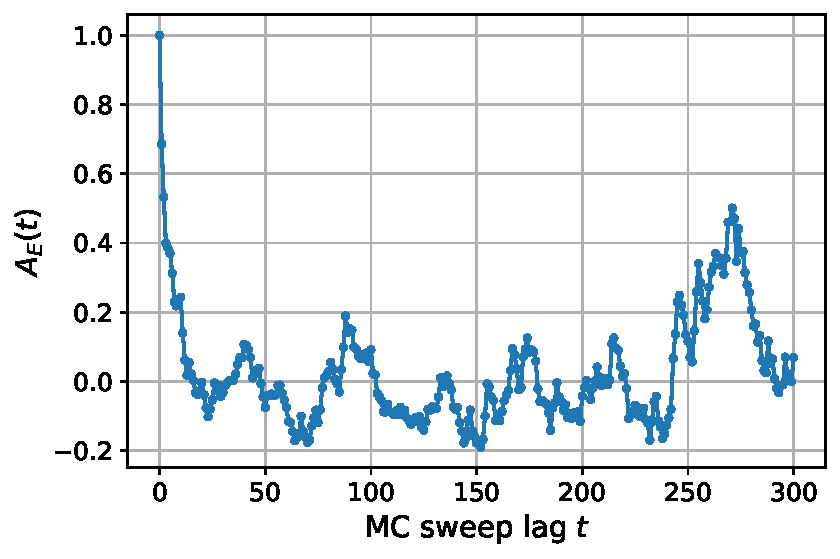
\includegraphics[width=\textwidth]{images/misc/autocorrfn_CIM.pdf}
    \end{subfigure}
    \caption{Energy density autocorrelation function $A_E(t)$ for $L = 128, \: T = 2.26$.}
\end{figure}
%%% FIG %%%

However, this natural estimator isn't \textit{quite} correct because the autocorrelations $A_\mathcal{O}(t)$ for $t \gg \tau_\text{int}$ contain much noise but little signal. To fix this, we implement the \textit{automatic windowing algorithm} \cite{Sokal1997} by introducing a cutoff $M$ on the sum
\begin{equation}
    \tau_{\text{int}, \mathcal{O}} = \frac{1}{2} + \sum_{t=1}^{M} A_\mathcal{O}(t)
\end{equation} 
$M$ is chosen as the smallest integer such that $M \geq 6 \tau_{\text{int}, \mathcal{O}}(M)$. The algorithm is summarized as follows  
\begin{enumerate}
    \setlength{\itemsep}{0.1em}
    \item Start with some small value of $M$, say $M=50$, and evaluate $\tau _{\text{int}, \mathcal{O}}(50)$.
    \item Check if $50 \geq 6\tau _{\text{int}, \mathcal{O}}(50)$.
    \item If not, increase the value of $M$ and repeat until you find a $M$ where $M \geq 6 \tau_{\text{int}, \mathcal{O}}(M)$.           
\end{enumerate}   
The autocorrelation time $\tau_\text{int}$ of a given $(L, T)$ configuration is the maximum of autocorrelation times for all observables except magnetization $m$ (due to lack of SSB in finite lattices). 
\begin{equation}
    \tau _\text{int} = \text{max}\:\{\tau_{\text{int},|m|},\: \tau_{\text{int}, m^2},\: \tau_{\text{int}, m^4},\: \tau_{\text{int}, E},\: \tau_{\text{int}, E^2}\}
\end{equation}
After running the preliminary MC run (Part 1) with measurements taken after every MC step to calculate the integrated autocorrelation time $\tau _\text{int}$, we perform the main MC run (Part 3) with measurements taken after every $2\tau _\text{int}$ steps.  

\section{Jackknife Analysis}
We begin by binning the $N$ measurements of observable $\mathcal{O}$ into $N_B$ non-overlapping bins of length $k$ such that $N_B k = N$, and construct a shorter time series of bin averages. The bin average for the $j^\text{th}$ bin is defined as
\begin{equation*}
    \mathcal{O}^{(B)}_j \equiv \frac{1}{k} \sum_{i = 0}^{k-1} \mathcal{O}_{jk+i} 
\end{equation*}
Below is a visual representation of the binning process 
\begin{gather*}
    \{\underbrace{\{\mathcal{O}_0, \mathcal{O}_1 \ldots \mathcal{O}_{k-1}\}}_{\overline{\mathcal{O}}^{(B)}_0}, \underbrace{\{\mathcal{O}_{k}, \mathcal{O}_{k+1} \ldots \mathcal{O}_{2k-1}\}}_{\overline{\mathcal{O}}^{(B)}_1}, \ldots\ldots ,\underbrace{\{\mathcal{O}_{(N_B-1)k}, \mathcal{O}_{(N_B-1)k+1} \ldots \mathcal{O}_{N-1}\}}_{\overline{\mathcal{O}}^{(B)}_{N_B-1}}\} \\
    \Downarrow \\
    \{
        \overline{\mathcal{O}}^{(B)}_0, \overline{\mathcal{O}}^{(B)}_1, \overline{\mathcal{O}}^{(B)}_2 \ldots ,\overline{\mathcal{O}}^{(B)}_{N_B-1} 
        \}
\end{gather*}
Knowing the bin averages for the observables $\mathcal{O} \in \{E, E^2, \abs{m}, m^2, m^4\}$, the bin estimates of the derived quantities are estimated as 
\begin{gather*}
    \chi^{(B)}_j = \beta \: L^2\:\qty(\overline{m^2}^{(B)}_j - \qty[\overline{|m|}^{(B)}_j]^2) \\[4pt] 
    {C_V}^{(B)}_j = \beta ^2\: L^2 \:\qty(\overline{E^2}^{(B)}_{\:\:\:j} - \qty[\overline{E}^{(B)}_j]^2) \\
    {U_L}^{(B)}_{\:\:\:j} = 1 - \frac{\overline{m^4}^{(B)}_j}{3\qty[\overline{m^2}^{(B)}_j]^2}
\end{gather*}
We denote these derived quantities by $\rho $ such that $\rho \in \{\chi , C_V, U_L\}$. The means over the bin averages (for $\mathcal{O}$) and bin estimates (for $\rho $) are also calculated
\begin{subequations}
    \begin{gather}
        \overline{\mathcal{O}} = \overline{\overline{\mathcal{O}}^{(B)}_j} = \frac{1}{N_B} \sum_{i=0}^{N_B-1} \overline{\mathcal{O}}^{(B)}_j \\
        \overline{\mathcal{\rho }} = \overline{{\rho }^{(B)}_j} = \frac{1}{N_B} \sum_{i=0}^{N_B-1} {\rho }^{(B)}_j
    \end{gather}       
    \label{binaverage} 
\end{subequations}
For the Jackknife error analysis, we begin by constructing the same number ($N_B$) of Jackknife bins containing all data but the $j^\text{th}$ bin of the previously mentioned binning method. The Jackknife averages for these new bins are defined as 
\begin{gather*}
    \overline{\mathcal{O}}^{(J)}_j = \frac{N\overline{\mathcal{O}} - k \overline{\mathcal{O}}^{(B)}_j}{N - k} \\
    \overline{\rho }^{(J)}_j = \frac{N\overline{\rho } - k {\rho}^{(B)}_j}{N - k}
\end{gather*}          
The error calculated using the Jackknife bins then comes out as
\begin{subequations}
    \begin{gather}
        \delta \overline{\mathcal{O}} = \sqrt{\frac{N_B-1}{N_B} \sum_{j=0}^{N_B-1}\qty(\overline{\mathcal{O}}^{(J)}_j - \overline{\mathcal{O}})^2} \\
        \delta \rho  = \sqrt{\frac{N_B-1}{N_B} \sum_{j=0}^{N_B-1}\qty(\overline{\rho }^{(J)}_j - \overline{\rho})^2}
    \end{gather}     
    \label{jackknifeerror}
\end{subequations}
\section{Simulation results}
The following parameters were used in the 2D Ising model simulations for lattice sizes of $L = 8, 16, 32, 64, 128$.  
\begin{itemize}[label={}]    
    \setlength{\itemsep}{0.1em}
    \item \textbf{For preliminary Monte Carlo (Part 1)}
    \begin{itemize}[label={}] 
        \setlength{\itemsep}{0.1em}   
        \item \texttt{no of equilibration sweeps = 1.0e3}
        \item \texttt{no of sampling sweeps = 1.0e4}
        \item \texttt{sampling step size = 1.0e0}
    \end{itemize} 
    \item \textbf{For the main Monte Carlo run (Part 3)}
    \begin{itemize}[label={}]    
        \setlength{\itemsep}{0.1em}
        \item \texttt{no of equilibration sweeps = 1.0e3}
        \item \texttt{no of sampling sweeps = 2$\tau \: \cdot$ 2.0e4}
        \item \texttt{sampling step size = 2$\tau $ }
    \end{itemize} 
\end{itemize}
%%% FIG %%%
\begin{figure}[!htb]
    \centering
    \begin{subfigure}[b]{0.47\textwidth}  %keep total sum <1 to show in same line
        \centering
        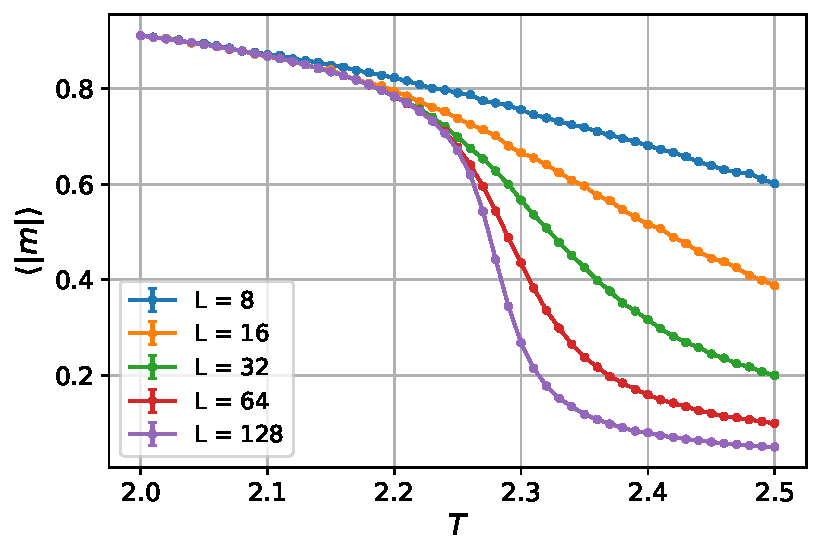
\includegraphics[width=\textwidth]{images/expval vs T/abs(mag).pdf}
        \caption{$\abs{M} \text{ vs } T$}
    \end{subfigure}
    \hspace{1em}  %\hfill
    \vspace{1em}
    \begin{subfigure}[b]{0.47\textwidth}
        \centering
        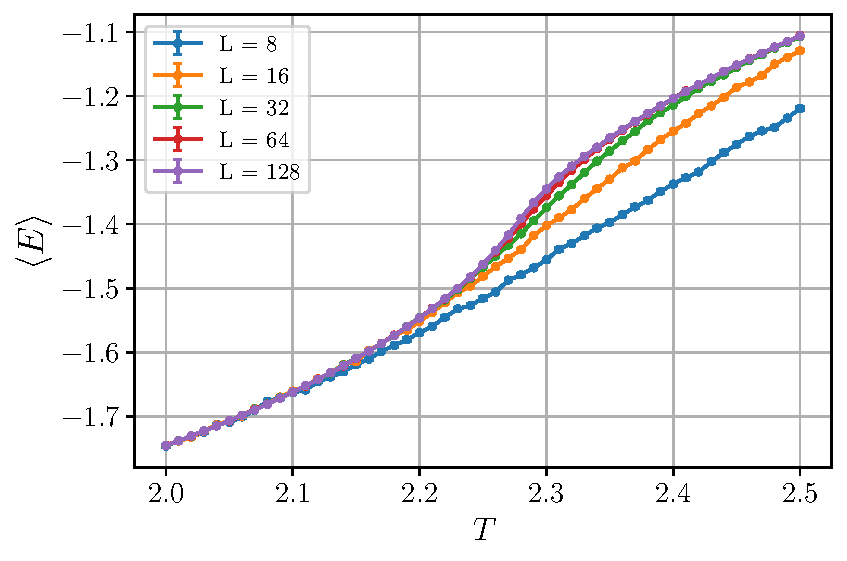
\includegraphics[width=\textwidth]{images/expval vs T/edens.pdf}
        \caption{$E \text{ vs } T$}
    \end{subfigure}
    \hspace{1em}  %\hfill
    \vspace{1em}
    \begin{subfigure}[b]{0.47\textwidth}
        \centering
        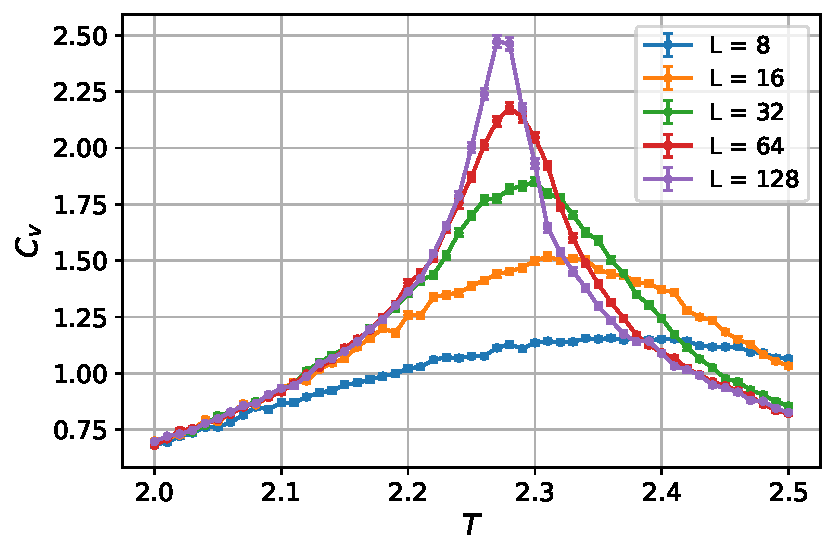
\includegraphics[width=\textwidth]{images/expval vs T/C_v.pdf}
        \caption{$C_V \text{ vs } T$}
    \end{subfigure}
    \hspace{1em}  %\hfill
    \begin{subfigure}[b]{0.47\textwidth}
        \centering
        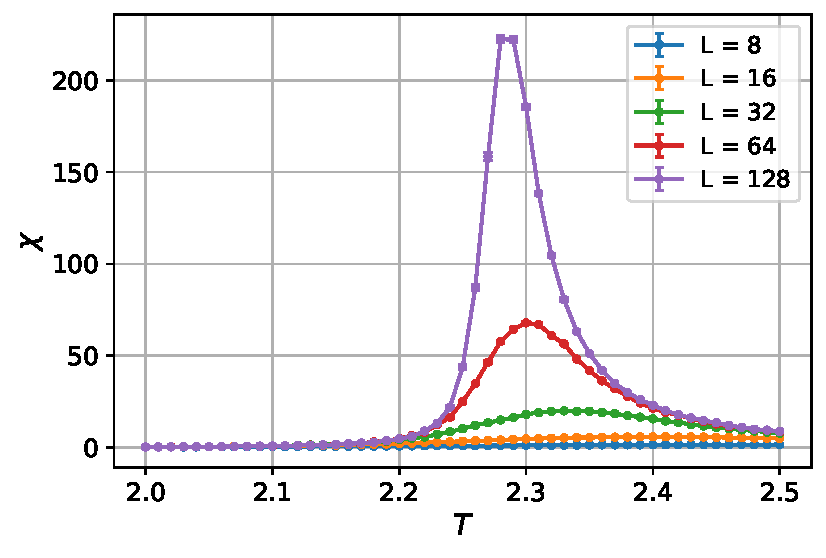
\includegraphics[width=\textwidth]{images/expval vs T/chi.pdf}
        \caption{$\chi \text{ vs } T$}
    \end{subfigure}
    \caption{Variation of physical quantities with $T$ for different lattice sizes $L$.}
    \label{expvalvsT}
\end{figure}
%%% FIG %%%

%%% FIG %%%
\begin{figure}[!htb]\ContinuedFloat
    \centering
    \begin{subfigure}[b]{0.47\textwidth}
        \centering
        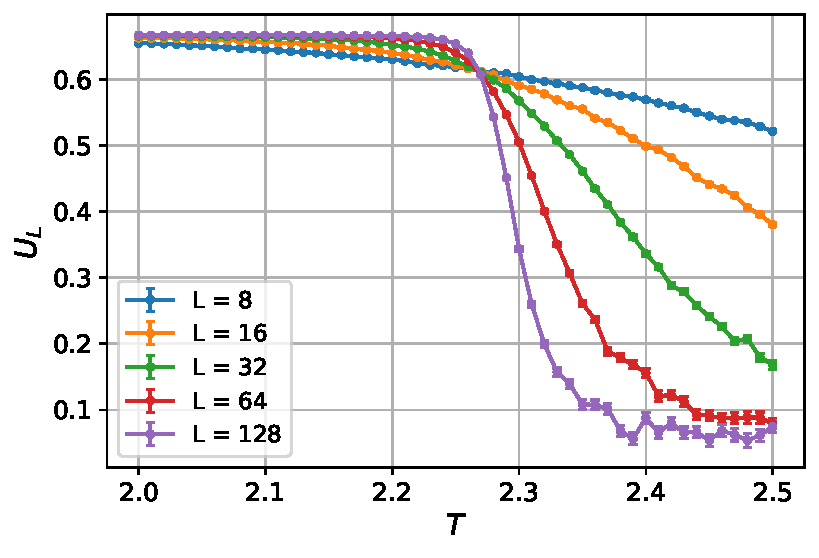
\includegraphics[width=\textwidth]{images/expval vs T/U_L.pdf}
        \caption{$U_L \text{ vs } T$}
    \end{subfigure}
    \hspace{1em}  %\hfill
    \begin{subfigure}[b]{0.47\textwidth}
        \centering
        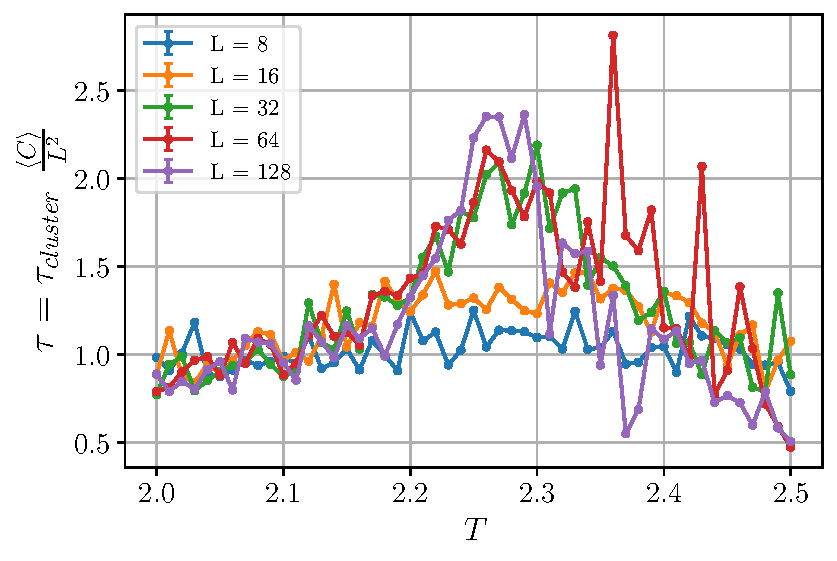
\includegraphics[width=\textwidth]{images/expval vs T/autocorr times.pdf}
        \caption{$\tau_\text{int} \text{ vs } T$}
    \end{subfigure}
    \caption{Variation of physical quantities with $T$ for different lattice sizes $L$.}
\end{figure}
\FloatBarrier
The Figure \ref{expvalvsT} above shows plots of expectation values of relevant observables, derived physical quantities and the autocorrelation times (scaled by $\expval{C}/L^2$) as they vary with $T$ for different lattice sizes $L$.~\\~\\
Furthermore, the critical temperature $T_c$ is obtained by finding the point of intersection of different $U_L$ vs $T$ curves, $\implies T_c \approx 2.269$.  

\section{Finite-size scaling}
According to the FSS hypothesis \cite{Sandvik_2010}, observables and derived physical quantities close to $T_c$ are a power of $L$ multiplied by a non divergent function of $tL^{1/\nu}$, i.e.
\[
    Q(t, L) = L^{\zeta/\nu} g(tL^{1/\nu}) 
\]
where $t = (T-T_c)/T_c$.
\begin{gather*}
    \text{\textbf{FS relations for 2D Ising model} } \\
    U_L =\:\:\: \: g_U(t L^{1/\nu}) \\ 
    |m| = L^{-\beta/\nu} \: g_{m}(t L^{1/\nu}) \\
    \chi = L^{\gamma/\nu} \: g_\chi(t L^{1/\nu}) \\
    C_V = \ln(L) \: g_C(t L^{1/\nu})
\end{gather*}
We use the \textit{data-collapse} method to estimate the critical exponents $\beta, \gamma$, and $\nu$ ($\alpha  = 0$ for 2D Ising model, so FSS hypothesis doesn't hold) by collapsing the curves corresponding to different lattice sizes $L$ on a single unknown master curve $g(x)$.~\\~\\
We use the following cost function $P_b$ to as a measure of the collapse, which is essentially a normalized sum of residues, which we get by slightly modifying the cost function given in \cite{Bhattacharjee_2001}.
\begin{equation}
    P_b = \frac{1}{N_\text{over}} \sum_p \sum_{j \neq p} \sum_i \frac{\qty|L_j^{-\zeta/\nu}Q_{ij} - \varepsilon_p\qty(L_j^{1/\nu} t_{ij})|}{L_j^{-\zeta/\nu}Q_{ij} + \varepsilon_p\qty(L_j^{1/\nu} t_{ij})}
\end{equation}    
\begin{itemize}
    \setlength{\itemsep}{0.1em}
    \item $p$ indexes the data-set associated to length $L_p$. 
    \item $j$ also indexes the data-set associated to length $L_j$, but doesn't include the set $p$.      
    \item $i$ indexes the data-points inside the set associated to $L_j$.   
    \item $N_\text{over}$ is the number of terms we sum over. 
\end{itemize} 
The critical exponents are obtained by minimizing the cost funtion $P_b$ with respect to $\beta, \gamma, \nu$, i.e. 
\begin{itemize}
    \setlength{\itemsep}{0.1em}
    \item $Q = U_L$, minimize $P_b(0, \nu)$ with respect to $\nu$. $\quad\longrightarrow \nu_0$
    \item $Q = |m|$, minimize $P_b(-\beta, \nu_0)$ with respect to $\beta$. $\quad\longrightarrow \beta_0$
    \item $Q = \chi$, minimize $P_b(\gamma, \nu_0)$ with respect to $\gamma$. $\quad\longrightarrow \gamma_0$   
\end{itemize}  

%%% FIG %%%
\begin{figure}[!htb]
    \centering
    \begin{subfigure}[b]{0.47\textwidth}  %keep total sum <1 to show in same line
        \centering
        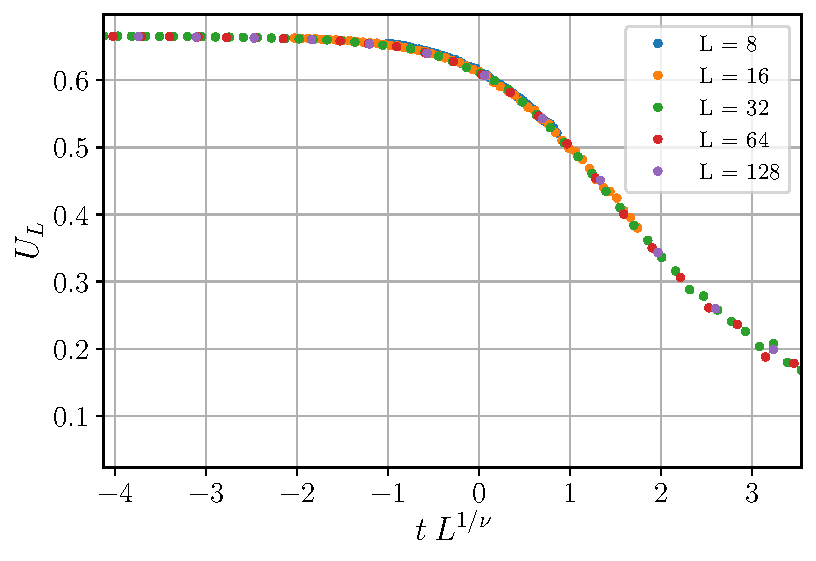
\includegraphics[width=\textwidth]{images/data collapse/U_L data collapse.pdf}
        \caption{Data collapse for $U_L$}
        \label{U_L collapse}
    \end{subfigure}
    \hspace{1em}  %\hfill
    \vspace{1em}
    \begin{subfigure}[b]{0.47\textwidth}
        \centering
        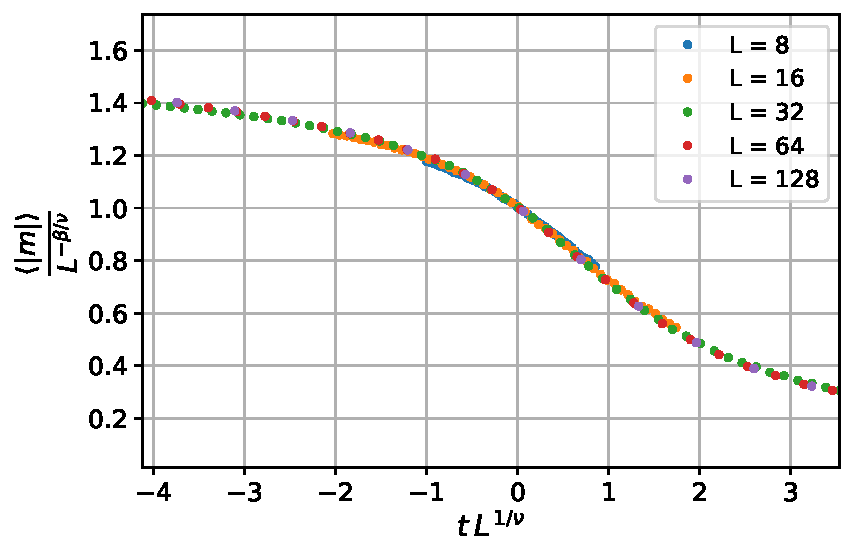
\includegraphics[width=\textwidth]{images/data collapse/abs(mag) data collapse.pdf}
        \caption{Data collapse for $\abs{M}$}
        \label{absmag collapse}
    \end{subfigure}
    \hspace{1em}  %\hfill
    \vspace{1em}
    \begin{subfigure}[b]{0.47\textwidth}
        \centering
        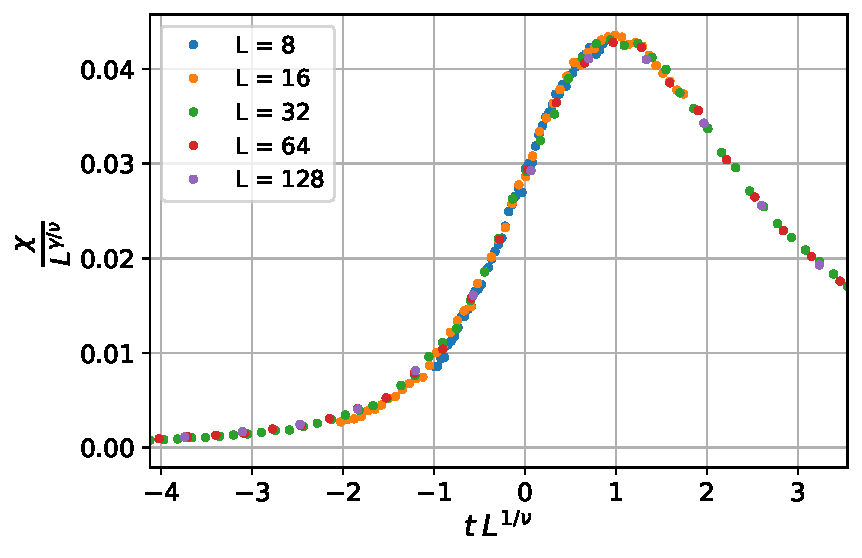
\includegraphics[width=\textwidth]{images/data collapse/chi data collapse.pdf}
        \caption{Data collapse for $\chi$}
        \label{chi collapse}
    \end{subfigure}
    \hspace{1em}  %\hfill
    \begin{subfigure}[b]{0.47\textwidth}
        \centering
        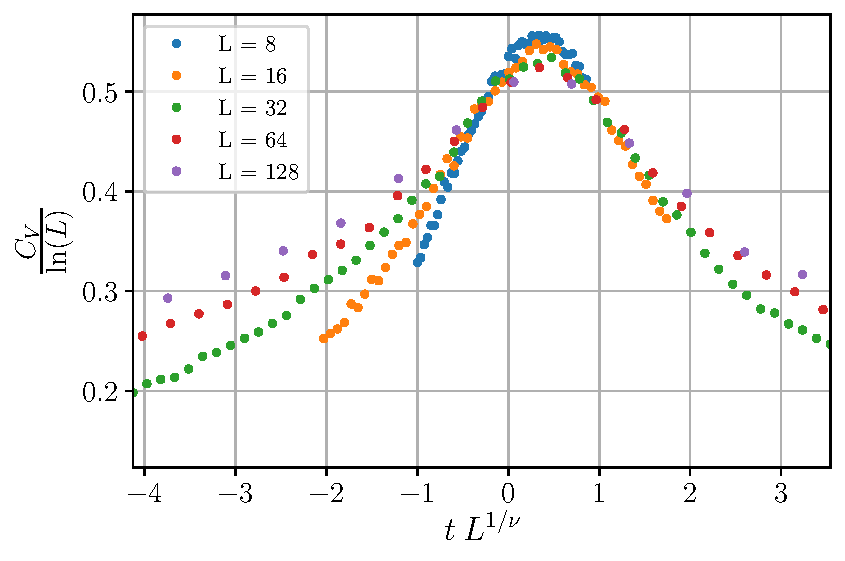
\includegraphics[width=\textwidth]{images/data collapse/C_v data collapse.pdf}
        \caption{Data collapse for $C_V$}
        \label{C_V collapse}
    \end{subfigure}
    \caption{Data-collapse to extract the critical exponents.}
    \label{datacollapse}
\end{figure}
The critical exponents estimated from the data collapse method are
\begin{equation*}
  \addtolength{\fboxsep}{5pt}
   \boxed{
    \begin{gathered}
        \nu = 0.9765 \\
        \beta = 0.1204 \\
        \gamma = 1.7301
    \end{gathered}
}
\end{equation*}

\subsection{The quality of data collapse (theory)}
The quality of the data collapse was defined as a reduced $\chi^2$ statistic by \cite{Houdayer_2004}, as follows 
\begin{equation}
    S = \frac{1}{\mathcal{N}} \sum_{i,j} \frac{(y_{ij} - Y_{ij})^2}{dy_{ij}^2 + dY_{ij}^2} ,
    \label{qualityfn}
\end{equation}
where the values $(y_{ij}, dy_{ij})$ are the scaled observations and its standard errors at $x_{ij}$, and the values $(Y_{ij}, dY_{ij})$ are the estimated value of the master curve and its standard error at $x_{ij}$.~\\~\\
The quality $S$ is the mean square of the weighted deviations from the master curve. As we expect the individual deviations $y_{i j}-Y_{i j}$ to be of the order of the individual error $\sqrt{d y_{i j}^{2}+d Y_{i j}^{2}}$ for an optimal fit, the quality $S$ should attain its minimum $S_{\min }$ at around 1 and be much larger otherwise.~\\~\\
Let $i$ enumerate the system sizes $L_{i}, i=1, \ldots, k$ and let $j$ enumerate the parameters $t_{j}, j=1, \ldots, n$ with $t_{1}<t_{2}<\ldots<t_{n}$. The scaled data are
$$
\begin{aligned}
y_{i j} &:=L_{i}^{-\zeta / \nu} Q_{L_{i}, t_{j}} \\
d y_{i j} &:=L_{i}^{-\zeta / \nu} d Q_{L_{i}, t_{j}} \\
x_{i j} &:=L_{i}^{1 / \nu} t_j
\end{aligned}
$$
The sum in the quality function $S$ only involves terms for which the estimated value $Y_{i j}$ of the master curve at $x_{i j}$ is defined. The number of such terms is $\mathcal{N}$.~\\~\\
The master curve itself depends on the scaled data. For a given $i, L_{i}$, we estimate the master curve at $x_{i j}$ by the two respective data from all the other system sizes which respectively enclose $x_{i j}$ : for each $i \neq i^\prime$, let $j^{\prime}$ be such that $x_{i^{\prime} j^{\prime}} \leq x_{i j} \leq x_{i^{\prime}\left(j^{\prime}+1\right)}$, and select the points $\left(x_{i^{\prime} j^{\prime}}, y_{i^{\prime} j^{\prime}}, d y_{i^{\prime} j^{\prime}}\right),\left(x_{i^{\prime}\left(j^{\prime}+1\right)}, y_{i^{\prime}\left(j^{\prime}+1\right)}, d y_{i^{\prime}\left(j^{\prime}+1\right)}\right)$. Do not select points for some $i^{\prime}$, if there is no such $j^{\prime}$. If there is no such $j^{\prime}$ for all $i^{\prime}$, the master curve remains undefined at $x_{i j}$.~\\~\\
Given the selected points $\left(x_{l}, y_{l}, d y_{l}\right)$, the local approximation of the master curve is the linear fit
$$
y=m x+b
$$
with weighted least squares. The weights $w_{l}$ are the reciprocal variances, $w_{l}:=1 / d y_{i j}^{2}$. The estimates and (co)variances of the slope $m$ and intercept $b$ are
$$
\begin{gathered}
\hat{b}=\frac{1}{\Delta}\left(K_{x x} K_{y}-K_{x} K_{x y}\right) \\
\hat{m}=\frac{1}{\Delta}\left(K K_{x y}-K_{x} K_{y}\right) \\
\hat{\sigma}_{b}^{2}=\frac{K_{x x}}{\Delta}, \hat{\sigma}_{m}^{2}=\frac{K}{\Delta}, \hat{\sigma}_{b m}=-\frac{K_{x}}{\Delta}
\end{gathered}
$$
with $K_{n m}:=\sum w_{l} x_{l}^{n} y_{l}^{m}, K:=K_{00}, K_{x}:=K_{10}, K_{y}:=K_{01}, K_{x x}:=K_{20}$, $K_{x y}:=K_{11}, \Delta:=K K_{x x}-K_{x}^{2}$
Hence, the estimated value of the master curve at $x_{i j}$ is
$$
Y_{i j}=\hat{m} x_{i j}+\hat{b}
$$
with error propagation
$$
d Y_{i j}^{2}=\hat{\sigma}^{2} x_{i j}^{2}+2 \hat{\sigma}_{b m} x_{i j}+\hat{\sigma}_{b}^{2} .
$$

\subsection{The quality of data collapse (results)}
Using the algorithm in the previous subsection, the quality of the different data collapse fits are as follows 
\begin{itemize}[label={}]
    \item Quality of $U_L$ vs $tL^{1/\nu}$ collapse $ = 1.6933$ (Fig. \ref{U_L collapse})
    \item Quality of $\expval{\abs{m}} L^{\beta/\nu}$ vs $tL^{1/\nu }$ collapse $ = 22.4764$ (Fig. \ref{absmag collapse})
    \item Quality of $\chi L^{-\gamma/\nu}$ vs $tL^{1/\nu}$ collapse $ = 0.7372$ (Fig. \ref{chi collapse})
    \item Quality of $C_V/\ln(L)$ vs $tL^{1/\nu}$ collapse $ = 6.9356$ (Fig. \ref{C_V collapse})      
\end{itemize} 

\section{Problems that I'm facing}
Following are some problems which I've not yet been able to resolve
\begin{enumerate}
    \item \textbf{Interpreting the quality of data collapse as error} \:\:\: As discussed in our last meeting, you mentioned that the reduced $\chi^2$ quality function $S$ (Eq. \eqref{qualityfn}) itself is a measure of an error after looking at \cite{Houdayer_2004}, so we can somehow normalize it to get the errors in physical quantities. However, even after reading the paper carefully, I still haven't understood how the authors calculated the errors, and to my knowledge, they haven't explicitly written down how they have calculated it.
\end{enumerate}

\end{document}